
\chapter{Pipeline Assembly in Python}
\label{chap:pipeline}
\subsection{Message passing}

\begin{figure}
    \centering
    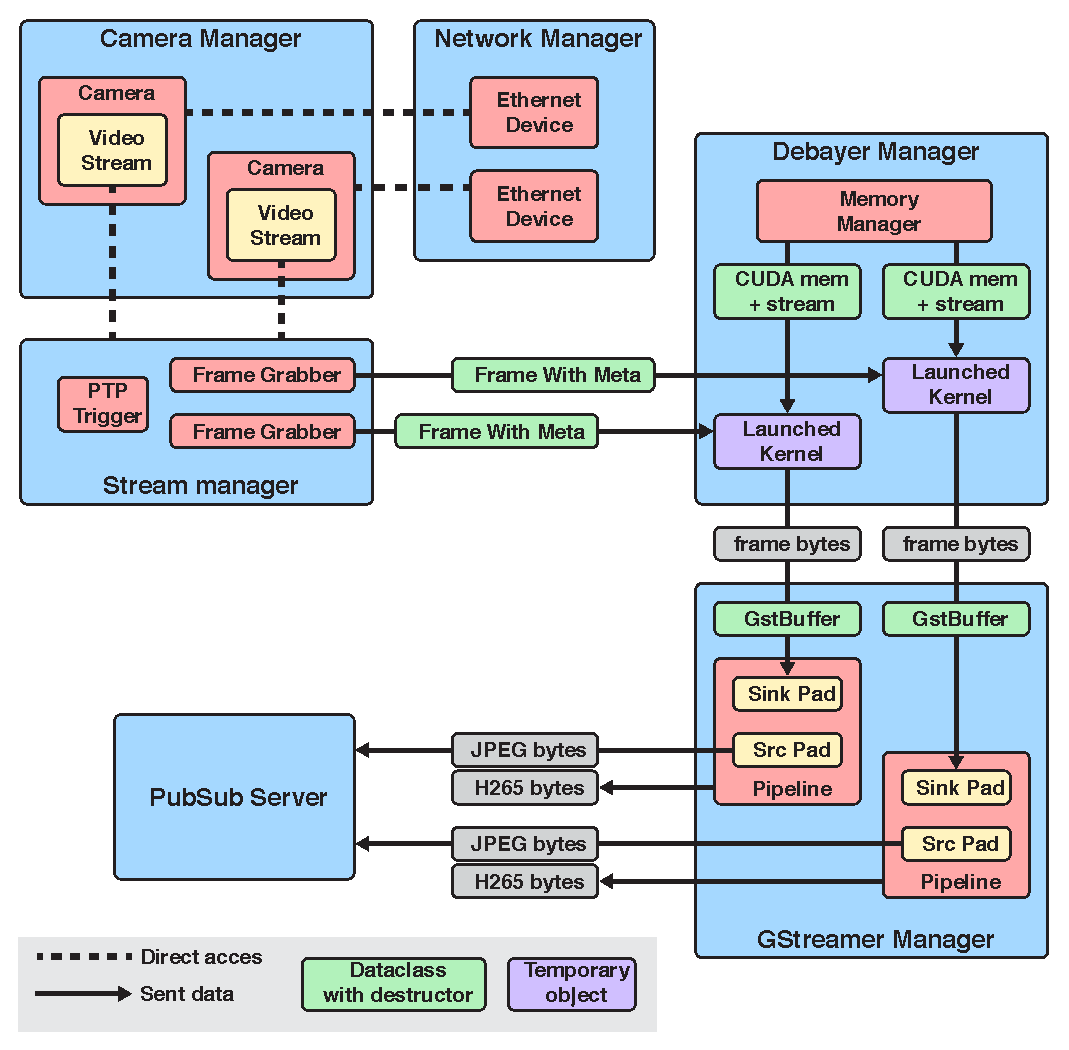
\includegraphics[width=\textwidth]{figures/object_overview.pdf}
    \caption{Class diagram showing the relationship between the classes in the pipeline and how thei interact.}
    \label{fig:pipeline_current}
\end{figure}

\subsection{Debayer Manager}
The main role of the debayer manager is to integrate the CUDA code with \py.
To acheive this \gls{pybind11} was used.
\gls{pybind11} is a \gls{cpp} library that allows for the creation of \py bindings for \gls{cpp}, also \gls{cpp} funcions that launch \gls{cuda} kernels.

Several ways are available to pass data between \gls{cpp} and \py, but when working with \gls{cuda} the easiest way is to pass pointers to \gls{numpy} or \gls{cupy} arrays, which are available trough the \code{__array_interface__} and \code{__cuda_array_interface__} respectively \cite{numpyArrayInterfaceProtocol} \cite{cupyInteroperabilityCuPy12}.
It is also possible to pass data as \gls{eigen}.

When working with \gls{pybind11} it is easiets to mamage the memory in \py and pass references to the \gls{cpp} code.

It is worth mentioning that it is also possible to write \gls{cuda} kernels in \py directly through \gls{cupy} as well as other \gls{gpu} accelerated libraries such as \gls{numba} and \gls{pytorch}
Based on prioer experience however these are impossible to debug and should be avoided for anything but the simplest of tasks.